\documentclass[a4paper,9pt]{extarticle}

%=========================================================
% PACKAGES
%=========================================================

\usepackage[
a4paper,
top=1.8cm,
bottom=1.5cm,
footskip=7mm,
left=1cm,
right=1cm,
headheight=14pt,
headsep=5mm
]{geometry}
\usepackage[T1]{fontenc}
\usepackage[utf8]{inputenc}
\usepackage[french]{babel}

\usepackage[sfdefault]{FiraSans}
\renewcommand{\familydefault}{\sfdefault}

\usepackage{multicol}
\setlength{\columnsep}{0.7cm}

\usepackage{amsmath,amssymb}

\usepackage{titlesec}
\usepackage{enumitem}

\usepackage{tcolorbox}
\tcbuselibrary{skins,breakable}

\usepackage{xcolor}

\usepackage{graphicx}
\usepackage{float}

\usepackage{tikz}

\usepackage{fancyhdr}
\usepackage[hidelinks]{hyperref}


%=========================================================
% PAGE SETTINGS
%=========================================================

\setlength{\parindent}{0pt}
\setlength{\parskip}{1.5pt}

\setlength{\abovedisplayskip}{4pt}
\setlength{\belowdisplayskip}{4pt}

\setlist[itemize]{
leftmargin=*,
itemsep=1pt,
topsep=1pt
}


%=========================================================
% COLORS
%=========================================================

\definecolor{Blue}{HTML}{E3F0FF}
\definecolor{Green}{HTML}{E3F7EA}
\definecolor{Pink}{HTML}{FFE5ED}
\definecolor{Orange}{HTML}{FFF0DC}
\definecolor{Purple}{HTML}{EEE7FF}
\definecolor{Yellow}{HTML}{FFFADB}


\definecolor{BlueTitle}{HTML}{285B8F}
\definecolor{GreenTitle}{HTML}{287052}
\definecolor{PinkTitle}{HTML}{A84063}
\definecolor{OrangeTitle}{HTML}{A96500}
\definecolor{PurpleTitle}{HTML}{6245A5}


%=========================================================
% HEADER
%=========================================================

\pagestyle{fancy}

\fancyhf{}

\fancyhead[L]{\small\textbf{Numerical Methods}}
\fancyhead[C]{\small Linear Systems I}
\fancyhead[R]{\small Week 02 --- 14-20/09/2026}

\fancyfoot[C]{\small\href{https://github.com/AlphaXT38G/notes_ba5}{github.com/AlphaXT38G/notes\_ba5}}
\fancyfoot[R]{\small \thepage}

\renewcommand{\headrulewidth}{0.4pt}



%=========================================================
% TITLES
%=========================================================

\titleformat{\section}
{\large\bfseries\color{BlueTitle}}
{}{0pt}{}

\titlespacing{\section}
{0pt}{6pt}{3pt}


% separator

\newcommand{\separator}{
\vspace{2pt}
\hrule
\vspace{3pt}
}


%=========================================================
% BOXES
%=========================================================

% Boxes are kept whole (unbreakable): inside multicols, a box split by tcolorbox
% leaves an empty column behind it.

% DEFINITION - blue
\newtcolorbox{definition}{
enhanced,
unbreakable,
colback=Blue,
colframe=BlueTitle,
boxrule=0.7pt,
arc=0mm,
title=\textbf{Definition},
fonttitle=\bfseries
}

% IMPORTANT - pink
\newtcolorbox{important}{
enhanced,
unbreakable,
colback=Pink,
colframe=PinkTitle,
boxrule=0.7pt,
arc=0mm,
title=\textbf{Key idea},
fonttitle=\bfseries
}

% FORMULAS - green
\newtcolorbox{formula}{
enhanced,
unbreakable,
colback=Green,
colframe=GreenTitle,
boxrule=0.7pt,
arc=0mm,
title=\textbf{Key formulas},
fonttitle=\bfseries
}

% WARNING - orange
\newtcolorbox{warning}{
enhanced,
unbreakable,
colback=Orange,
colframe=OrangeTitle,
boxrule=0.7pt,
arc=0mm,
title=\textbf{Warning},
fonttitle=\bfseries
}

% EXAMPLE - purple
\newtcolorbox{example}{
enhanced,
unbreakable,
colback=Purple,
colframe=PurpleTitle,
boxrule=0.7pt,
arc=0mm,
title=\textbf{Example},
fonttitle=\bfseries
}

% SUMMARY - orange
\newtcolorbox{summary}{
enhanced,
unbreakable,
colback=Yellow,
colframe=OrangeTitle,
boxrule=0.7pt,
arc=0mm,
title=\textbf{Summary},
fonttitle=\bfseries
}



%=========================================================
% FIGURE BOX
%=========================================================

\newtcolorbox{figurebox}{
enhanced,
colback=white,
colframe=gray,
boxrule=0.5pt,
arc=0mm,
center
}



%=========================================================
% DOCUMENT
%=========================================================

\begin{document}

%\footnotesize   --> To reduce the size of the text

\thispagestyle{fancy}



% Columns keep their natural height: boxes are unbreakable, stretching would open gaps.
\raggedcolumns
\begin{multicols}{2}


%=========================================================
\section{From Numbers to Vectors and Matrices}


Recap of lecture 1: we understand how floating point arithmetic generally works (play with
formats on \href{https://evanw.github.io/float-toy/}{Float Toy}). \textbf{But} individual numbers
aren't enough: real problems involve millions to billions of numbers arranged in specific ways.
Today: the most common arrangement, \emph{vectors \& matrices}.


\begin{definition}

\textbf{SCALARS, VECTORS, MATRICES, TENSORS}

Key numerical data structures organized by dimension: scalar, row vector, column vector, matrix,
tensor. All are \textbf{nd-arrays} (general n-dimensional storage); vectors and matrices are
representations of \emph{linear functions}.

\end{definition}


\begin{definition}

\textbf{LINEAR FUNCTION}

$f$ is a linear function \emph{if and only if}

\begin{align*}
f(\mathbf{x} + \mathbf{y}) &= f(\mathbf{x}) + f(\mathbf{y}) && \text{(additivity)} \\
f(\alpha\mathbf{x}) &= \alpha f(\mathbf{x}) \quad (\alpha \in \mathbb{R}) && \text{(homogeneity)}
\end{align*}

In this case $f(\mathbf{x}) = \mathbf{A}\mathbf{x}$ fully encodes everything that $f$ does!

\end{definition}


\begin{formula}

\textbf{Matrix-vector multiplication}

\[
(\mathbf{A}\mathbf{x})_i = \sum_{k=1}^{n} A_{ik} x_k
\]

With the columns $\mathbf{a}^{(1)}, \mathbf{a}^{(2)}, \mathbf{a}^{(3)}$ of $\mathbf{A}$:

\[
\mathbf{A}\mathbf{x} = \mathbf{a}^{(1)} x_1 + \mathbf{a}^{(2)} x_2 + \mathbf{a}^{(3)} x_3
\]

a linear combination of the columns (if they are linearly dependent, they span e.g.\ only a 2D
subspace).

\end{formula}


\textbf{Basic matrix transformations in 2D}

\begin{center}

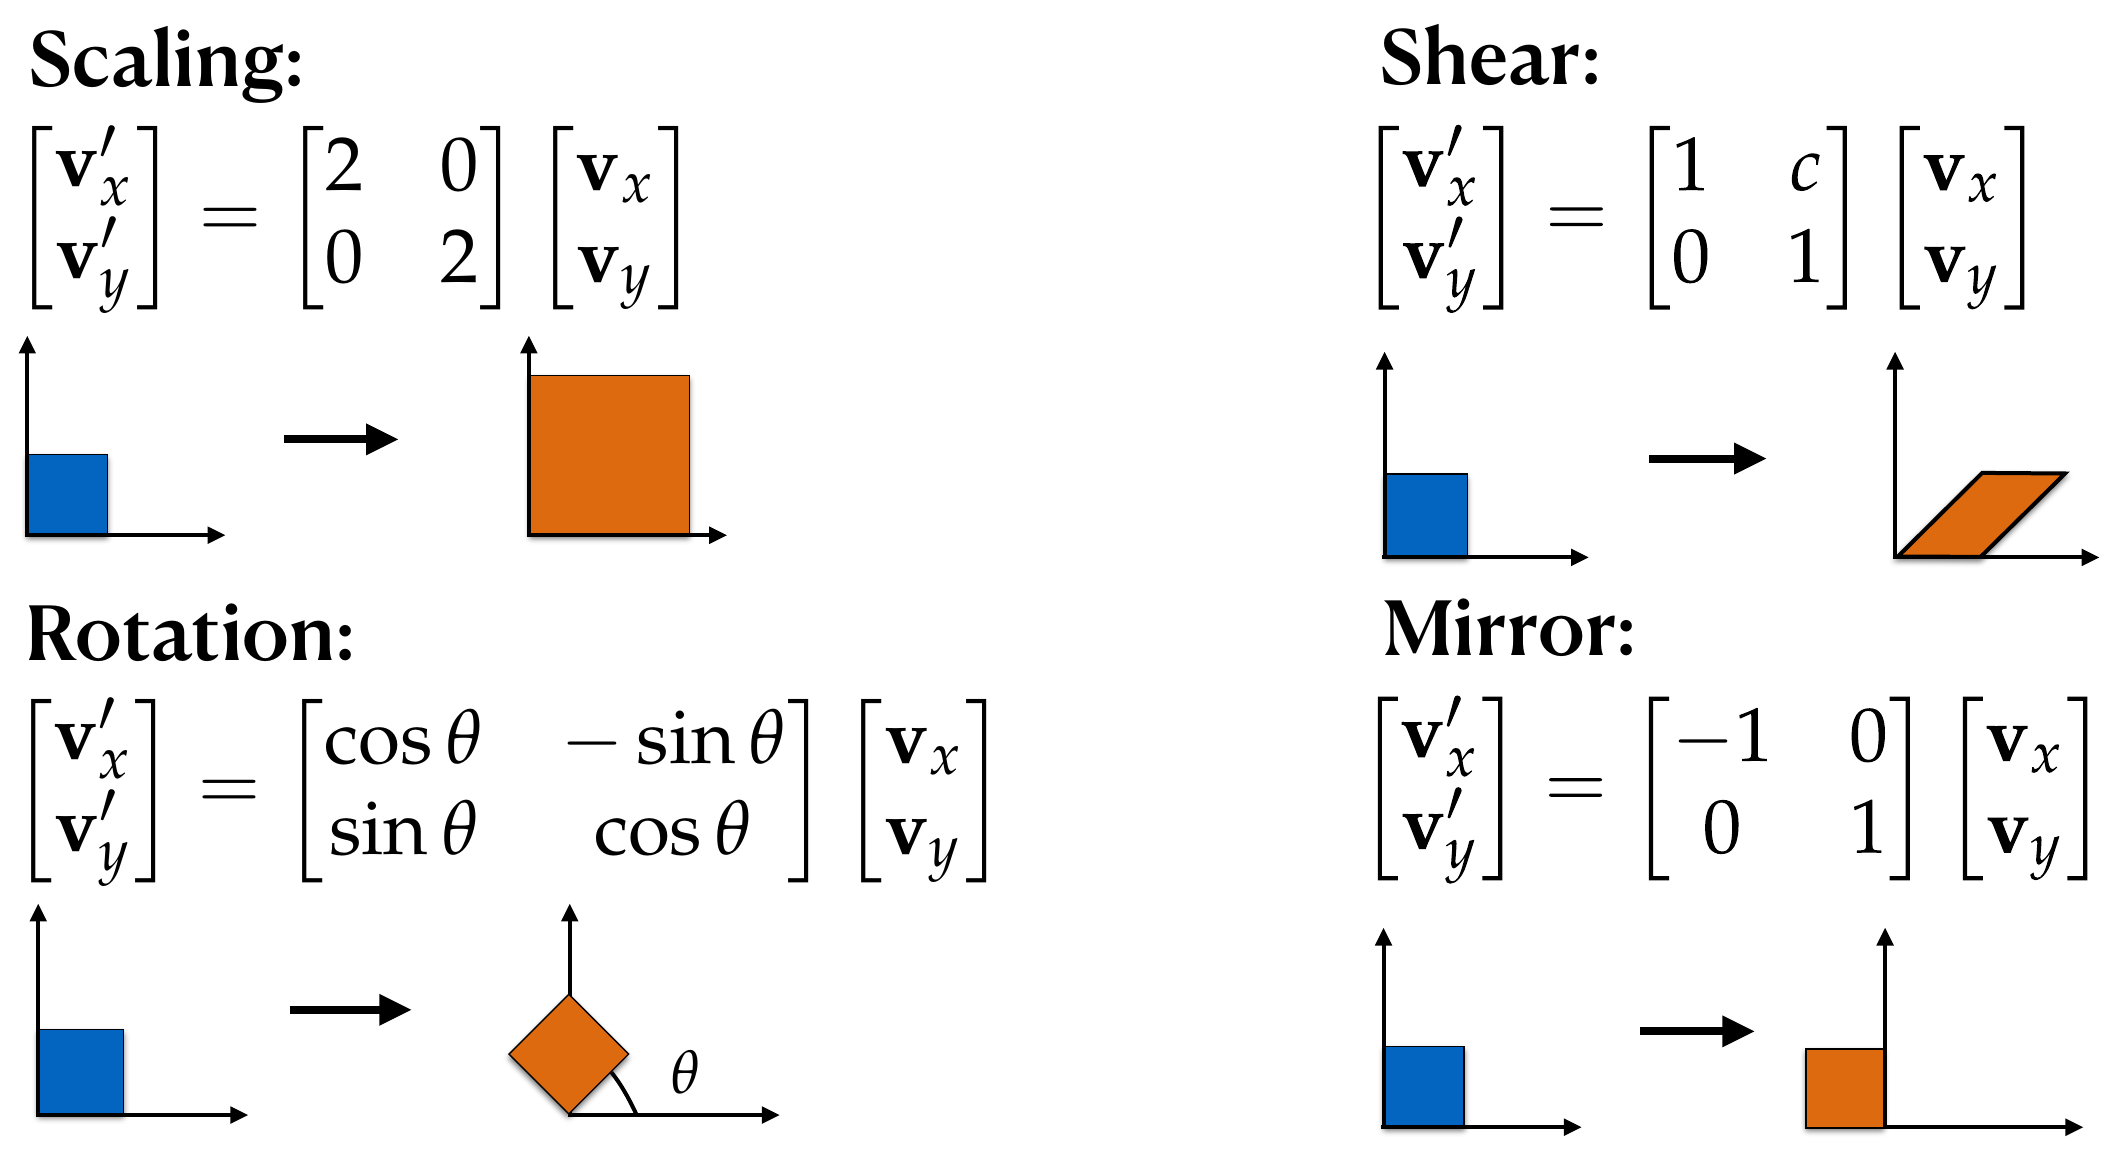
\includegraphics[
width=0.85\linewidth
]{../images/week02_01.png}

\end{center}


\begin{important}

\textbf{Why care about linear functions?}

\begin{itemize}

\item Solving linear problems is one of the (few) numerical problems that we know to solve
\textbf{really well}: when you can turn something into a linear system, good job, you are done.
\emph{Nonlinear} methods are \emph{fragile}.

\item Almost everything boils down to a linear system at some point.

\end{itemize}

\end{important}


\textbf{Course topics} (``veggies first, then the cake''): 1.\ floating point arithmetic \& error;
2.\ linear systems, LU (\emph{today}); 3.\ conditioning \& least squares basics; 4.\ least squares,
QR; 5.\ writing efficient numerical code; 6.\ eigenanalysis, SVD; 7.\ nonlinear problems; 8.\
automatic differentiation; 9.\ neural networks.



\end{multicols}


\end{document}
